\documentclass{oblivoir}
\usepackage{amsthm}
\usepackage{thmtools}

%\usepackage{ansform}
\usepackage{ikps}

\declaretheoremstyle[% spaceabove=6pt,spacebelow=6pt, headfont=\color{MainColorOne}\sffamily\bfseries, notefont=\mdseries, notebraces={[}{]}, bodyfont=\normalfont,
headpunct={},
postheadspace=1em,
%qed=▣,
]{maintheorem}

\declaretheorem[%
name=정의,
style=maintheorem,
numberwithin=section, shaded={%bgcolor=MainColorThree!20,
margin=.5em}]{dfn}
% \begin{dfn}[]
% \end{dfn}

\newtheorem{theorem}{Theorem}[section]
\newtheorem{corollary}{Corollary}[theorem]
%https://www.overleaf.com/learn/latex/Theorems_and_proofs
%http://web.mit.edu/rsi/www/pdfs/theorems.pdf
%https://texfaq.org/FAQ-proof
\declaretheorem[%
name=정리,
style=maintheorem,
numberwithin=section, shaded={%bgcolor=MainColorThree!20,
margin=.5em}]{thm}

%\newcommand{}[][]{}
\setcounter{secnumdepth}{3}
%https://tex.stackexchange.com/questions/130795/how-can-i-number-sections-below-subsection-in-latex


\begin{document}

\tableofcontents


\section{GRAPHS AND SUBGRAPHS}
\subsection{Graphs and simple Graphs}

\begin{dfn}[Graph] 정점과 정점을 잇는 간선들로 이루어진 것을 그래프라한다.
    \begin{itemize}
        \item $V(G)$ :  정점의 집합
        \item $E(G)$ :  간선의 집합
        \item $\psi_G(e_n)$ :  각 간선($e_n$)의 정점의 쌍
        \item $\nu(G)$ :  정점의 갯수 
        \item $\varepsilon(G)$ :  간선의 갯수
    \end{itemize}

    
    그래프를 간선들이 교차하지않게 그릴수 있는 것을 plannar graph라 한다. plannar graph가 아닌 것을 nonplanar graph라한다.
    
    정점이 한개인 그래프를 trivial graph라고 한다. 이외의 모든 그래프는 nontrivial 그래프이다.

    Simple graph : loop가 없고 두 정점쌍에 두개이상의 간선이 존재하지않는 그래프

    incident : 한 간선에 양 정점 근접
    adjacent : 두 간선에 공통된 정점 인접

    
\end{dfn}

\subsection{Graph Isomorphism}

\begin{dfn}[isomophic] 두 그래프 G와 H가  전단사 함수 $\theta : V(G) \longrightarrow V(H)$와 $\phi : E(G) \rightarrow E(H)$이 성립하면 두 그래프는 동형(isomophic)이다.
    또한 다음이 성립한다.
\begin{itemize}
    \item $\psi(e) = us( e \in E(G), u,s \in V(G)) $
    \item $\psi(\phi(e)) = \theta(u)\theta(v)$% $\phi(e)$ %($\phi(e) \in E(H)$)
\end{itemize}
\end{dfn}

\begin{dfn}[a special classes of graphs] 특징에 따른 그래프 이름
    \begin{itemize}
        \item complete graph(완전 그래프) : 모든 정점에 간선이 연결된 그래프 정점의 개수가 $n$일때 $K_n$로 표현한다.
        \item empty graph : 정점이 한개고 간선이 없는 그래프
        \item bipartite graph(이분 그래프) : 정점이 두 집합으로 이루어져 집합 내에는 연결된 간선이 없는 그래프
        \item complete bipartite graph(완전 이분 그래프) : 한 집합의 모든 정점이 각각 반대 집합의 모든 정점에 연결된 그래프 두 정점 집합의 갯수가 각각 $m$과  $n$일때 $K_{m,n}$으로 표현한다.
        \item (1.2.9)k-partite graph : 정점이 적어도하나 포함된 k개의 부분 집합으로 이루어진 그래프이다  한 부분집합 내에 연결된 간선은 존재하지 않고 다른 부분집합의 정점에만 간선이 존재할수있다.
        (원문)a complete k-partite graph is one that is simple and in which each vertex is
        joined to every vertex that is not in the same subset
        \item (1.2.9)complete k-partite graph : k-partite graph의 각 정점이 포함된 부분집합을 제외한 모든 정점에 간선이 연결된 그래프 
        
        (원문)complete k-partite graph is one that is simple and in which each vertex is
        joined to every vertex that is not in the same subset.

        \item (1.2.10)k -cube : 각 정점은 하나의 ordered k-tuple(k-비트 이진수)이고, 두 정점이 1비트만 서로 다를 때 두 정점간에 에지가 있다.
        \item (1.2.11)여 그래프(complement graph) : 모든 정점에 대해서 포함하고 있는 존재하는 간선은 제거, 존재하지않는 간선을 생성해서 만든 그래프 
        $G^{c}$로 표현한다.
        \item (1.2.11)자기 여 그래프 (self-complementary graph) : 여그래프와 자기자신이 동형인 그래프
    \end{itemize}
\end{dfn}

week1

\subsubsection{}
\subsubsection{}
\subsubsection{}
\subsubsection{}
\subsubsection{} %1.2.5
$G \cong H$ , simple

bijection $\theta : V(G) \longrightarrow V(H)$
$ uv \in E(G) \Leftrightarrow  \theta(u)\theta(v) \in E(H)$

정의로 부터 $\psi(e) = us$인 간선 $e$ ($e \in E(G)$)에 대해 대응되는 $\psi(\phi(e)) = \theta(u)\theta(v)$인 $\phi(e)(\phi(e) \in E(H))$가 존재함을 알 수 있다. 
따라서 $ uv \in E(G) \rightarrow \theta(u)\theta(v) \in E(H)$ 성립, 반대의 경우도 마찬가지로 성립한다.

\subsubsection{}
\subsubsection{}
\subsubsection{}
\subsubsection{}%1.2.9

\begin{align}
&{n \choose 2} -  (m(k+1)-n) {k \choose 2} -(n-mk){k+1 \choose 2} \\
&= {n \choose 2} -  m(k+1){k \choose 2}-n{k \choose 2} -(n-mk){k+1 \choose 2} \\
&= {n \choose 2} -  m(k-1){k+1 \choose 2} +n{k \choose 2} -(n-mk){k+1 \choose 2} \\
&= {n \choose 2} + n{k \choose 2} -(n-m){k+1 \choose 2} \\
&= {n \choose 2} + n{k \choose 2} -(n-m){k+1 \choose 2} +(n-1){k+1 \choose 2} - (n-1){k+1 \choose 2}\\
&= {n \choose 2} + n{k \choose 2} - (n-1){k+1 \choose 2} + (m-1){k+1 \choose 2}  \\
&= \dfrac{n^2-n-nk + k^2+k-nk}{2}  + (m-1){k+1 \choose 2} \\
&= \dfrac{(n-k)(n-k-1)}{2}={n-k \choose 2}  + (m-1){k+1 \choose 2}
\end{align}

\subsubsection{}
\subsubsection{}
%1.2.11
(a):
\begin{itemize}
    \item $K_{n}^{c}$ : 간선이 없는 그래프이다.
    \item $K_{n,m}^{c}$ : 두 집합사이의 간선이 없이 두 집합이 각각 완전그래프인 subgraph를 이루고있다.
\end{itemize}
(b): 자기 여 그래프가 되기위해선 일단 동형 이전에 간선의 갯수가 동일해야하는데 여기서 총 생길수있는 간선의 갯수는 $\dfrac{v(v-1)}{2}$가 최댓값이자 그래프의 간선수 + 여그래프의 간선수 입니다. 그래프의 간선수 = 여그래프의 간선수 이므로 $v$나 $v-1$은 적어도 둘 중 하나는(적어도지만 사실 둘다 4의 배수인 경우의 수는 존재하지않습니다) 4의 배수여야합니다 따라서 $v\pmod{4}$는 0 또는 1


\begin{itemize}
\item 추가문제 :

인접성 : 두 그래프가 인접성을 보존할때, $u$와 $v$가 인접하면 $\theta(u)$와  $\theta(v)$가 인접하고 그 역도 성립한다. 

두 그래프 G와 H에 대해서 G의 정점들을 H의 정점들에 일대일로 대응하면서 
인접성을 보존하는 함수 f가 존재하면 두 그래프 G와 H는 동형(isomorphic)이다.

Proof: $E(G)$의 임의의 간선 $e$에 대해 임의의 정점 $u,v$가 인접할때, 인접성이 보존되므로 $\theta(u)$와  $\theta(v)$ 또한 인접한다.
$\theta(u)$와  $\theta(v)$를 잇는 간선을 $e'$이라 할때 $\phi(e) = e'$인 $\phi: E(G) \longrightarrow E(H)$를 정의할 수 있다.
따라서 정의에 의해 $G$와 $H$는 동형이다.
\end{itemize}

week2

\subsection{The Incidence and Adjacency Matrices}
(대충 그래프를 나타내는 표현에 대한 내용)
\subsection{Subgraphs}
\begin{dfn}[subgraph]
    그래프 $H$, $G$가 $ V(H) \subset V(G), E(H) \subset E(G)$, and $\psi_{H}$ is restricton $\psi_{G}$ \protect\footnote{$\psi_{H}$가 제한적으로 $\psi_{G}$이다.} 일때  $H \subseteq G$ 라쓰고 $H$($G$)를 subgraph(supergraph)라 한다.

    \begin{itemize}
        \item $H \subseteq G$,$H\neq G $이면 $ H \subset G$라 표기하고, $H$를  $G$의 proper graph라 한다.
        \item $V(H) = V(G) , H \subseteq G $이면 $H$($G$)를  spaning subgraph(supergraph)라 한다.
        \item spaning subgraph과 동시에 simple graph이면, undelying simple graph라한다.
    \end{itemize}
\end{dfn}
\subsection{Vertex Degrees}
\begin{dfn}[degree(차수)] $d_G(v)$는 정점 $v$에 연결된 간선의 갯수를 나타낸다. 그래프의 정점의 차수의 최솟값을 $\delta(G)$ , 최댓값을 $\Delta(G)$로 표기한다.
    \[
        \sum_{v \in V} d(v) = 2 \varepsilon  
    \]
    k-regular graph(정규그래프) : $d(v) = k \:\forall v \in V$
    $|A|$ : 집합 $A$의 원소의 갯수
\end{dfn}

\begin{theorem}
    \[
        \sum_{v \in V} d(v) = 2\varepsilon  
    \]
\end{theorem}

\begin{proof}
    근접행렬 $M$을 생각해보자 각 열은 정점으로 이루어져있으므로 행의 합은 해당 정점의 차수이다. 따라서 모든 행과 열의 합은 $\sum_{v \in V} d(v)$이며 또한 $2\varepsilon $이다. 예제 1.3.1(a)에 따라서 각 열의 합이 2이다. 
\end{proof}

\begin{corollary}
    어떤 그래프의 차수가 홀수인 정점의 갯수는 짝수이다.
\end{corollary}

\begin{proof}
    차수가 홀수와 짝수인 $V_1$, $V_2$로 정점을 나누었을 때,
    \[
        \sum_{v \in V_1} d(v) + \sum_{v \in V_2} d(v) = \sum_{v \in V} d(v)
    \]
    는 짝수이다. $\sum_{v \in V_2} d(v)$는 짝수이므로 $\sum_{v \in V_1} d(v)$ 또한 짝수이다. 그러므로 $|V_1|$은 짝수이다.
\end{proof}

\subsubsection{}
\subsubsection{} 
%1.5.2
M'는 M의 전치행렬 원표기 $M^{T}$,
$MM'[v_i][v_i] = \sum_{j=1}^n M[v_i][e_j] \cdot M'[e_j][v_i]$

$ M'[e_j][v_i] = M[v_i][e_j] $이며 simple graph일때 각 값은 0 또는 1이기 때문에 결과적으로 대각선의 값은 해당 정점의 차수가 된다.

$A$ 행렬에서 $A[v_i][v_j] = A[v_j][v_i]$ 

$d(i) = \sum_{j=1}^n A[v_i][v_j] = \sum_{j=1}^n A[v_j][v_i]$이다.
마찬가지로 simple graph에서 $A[v_i][v_j]$은 무조건 0 또는 1을 가지므로 $A[v_i][v_j] \cdot A[v_j][v_i] = A[v_i][v_j]$이다.

$A^2$에서 $A^2[v_i][v_i] = \sum_{j=1}^n A[v_i][v_j] \cdot A[v_j][v_i]= \sum_{j=1}^n A[v_i][v_j] = d(i)$

\subsubsection{} 
% 1.5.3

k-regular bipartite graph의 bipartition($X$,$Y$)이 $|X|\neq |Y|$라 하자. $d(v)=|Y|,\: d(u)=|X|(v \in X, u \in Y )$ $d(v) \neq d(u)$ 이는 k-regular graph의 조건에 모순

\subsubsection{} 
% 1.5.4

두명 이상의 사람이 있는 그룹에서 그룹 내 친구의 수(그룹 내부의 사람으로 제한)가 같은 사람이 반드시 두명이 있음을 보여라

사람이 n명일때 친구의 수는 최대 n-1명이기때문에 비둘기집의 원리에 의해 친구 수가 같은 사람이 무조건 두명이 존재한다.

각각의 사람을 정점, 친구관계를 간선으로 나타낸다면은 해당 그룹은 simple graph로 볼수있으며 친구의 수는 각 정점의 차수가 된다.

따라서 해당 문제는 simple graph일때 반드시 두 정점의 차수가 같음을 보이는 것과 같다. 
\subsubsection{} 
% 1.5.5
만약 $G$가 정점 $v_1, v_2, ... , v_n$을 가질때 $(d(v_1), d(v_2), ... , d(v_n))$ 을 그래프 $G$의 차수 수열(degrees sequence)라 부른다.

음이 아닌 정수들의 시퀀스 $(d_1, d_2, ... , d_n)$가 어떤 그래프의 차수 시퀀스임이 $\sum_{i=1}^n d_i$가 짝수임과 필요충분 조건임을 보여라.

그래프의 차수의 합은 $2\varepsilon$임이  $Theorem1.1$에 이미 증명되어 있다. 따라서 차수 수열의 합은 짝수이며 반대의 경우도 성립한다.


If G has vertices $(v_1, v_2, ... , v_n)$ the sequence $(d(v_l), d(v_2), ... , d(v_n))$ is called a degree sequence of G. 
Show that a sequence $(d_1, d_2, ... , d_n)$ of non-negative integers is a degree sequence of some n
graph if and only if $\sum_{i=1}^n d_i$ is even

\subsubsection{} 
% 1.5.6 
    A sequence $d = (d_1, d_2 , ... , d_n)$ is graphic if there is a simple graph with degree sequence d. Show that

(a) (7,6,5,4,3,3,2) : 정점이 총 7갠데 첫번째 정점의 간선이 7개인것은 simple graph의 조건을 충족하지 못한다.
(6,6,5,4,3,3,1) : 총 7개의 정점중 자신을 제외한 모든 정점에 간선을 잇는 차수가 6인 정점이 2개이지만 차수가 1인 정점이 있으므로  simple graph임이 모순이다.

(b) if $d$ is graphic and $d_1 \le d_2 \le ... \le d_n$, then $\sum_{i=1}^{n} d_i$ is even and $\sum_{i=l}^{k} d_i \le k(k -1)+\sum_{i=k+1}^{n}\min(k, d_i)$ for $1 \le k \le n$

그래프가 심플그래프일때 차수 수열이 $d_1 \le d_2 \le ... \le d_n$이면,  $\sum_{i=1}^{n} d_i$ 짝수인것과 다음이 성립함을 보이시오
$\sum_{i=1}^{k} d_i \le k(k -1)+\sum_{i=k+1}^{n}\min(k, d_i)$ for $1 \le k \le n$

d는 차수수열이므로 d의 합은 $2\varepsilon$이다.
\subsubsection{} 
%
\subsubsection{} 
%
\subsubsection{} 
%
\subsubsection{} 
%1.5.10

The edge graph of a graph G is the graph with vertex set E(G) in
which two vertices are joined if and only if they are adjacent edges in G. 

Show that, if G is simple
(a) the edge graph of G has e(G) vertices and L (d2 (V)) edges; vEVlG) .
(b) the edge graph of Ks is isomorphic to the complement of the graph featured in exercise 1.2.6.

그래프 G의 엣지 그래프는 꼭지점 집합 E (G)가있는 그래프로 두 개의 꼭지점이 G의 인접 엣지 인 경우에만 결합됩니다.

\subsection{Paths and Connection}
\begin{dfn}[walk]순차적으로 이어지는 정점, 간선의 연결을 walk라한다. $v_{0}e_{1}v_{1}e_{2}v_{2} ... e_{k}v_{k}$인 walk를 $v_0$ to $v_k$ 또는 ($v_0$, $v_k$)-walk라 한다.
    \begin{itemize}
        \item 지나는 간선을 한번씩만 쓴 walk를 trail이라한다.
        \item simple graph $G$의 모든 간선을 지나는 trail의 길이는 $\varepsilon (W)$이다.
        \item 지나는 정점을 한번씩만 쓴 walk를 path라 한다
        \item 그래프 G가 두 정점 u,v의  (u,v)-path가 존재할때, connected graph라한다.
        \item 그래프의 정점을 쪼갠 부분 그래프들이 모두 각각의 연결된 그래프일때, 부분 그래프들을 그래프 G의 component라 한다.
        \item 그래프 G의 componet의 수를 $\omega(G)$라 쓴다.
    \end{itemize}
\end{dfn}
\subsubsection{} 
% 1.6.1 

($u$,$v$)-walk사이에 사이클이 존재 할 경우 겹치는 정점을 중복사용하지않는 walk를 짤수있다 따라서 ($u$,$v$)-path가 존재한다.
\subsubsection{} 
%1.6.2
????

\subsubsection{} 
%1.6.3
한 정점을 패스의 시작정점으로 잡았을때 $\delta \le k$ 이기때문에  lenth가 $k$인 path를 만들기위해 서로 다른 $k$개의 연결된 정점을 선택해 path를 생성할수있다.
\subsubsection{} 
% 1.6.4
????
\subsubsection{} 
%1.6.5
(a) : 최대한 적은 정점에 많은 간선을 사용한 그래프를 세팅하기위해,  정점 하나를 제외한 $\varepsilon-1$개의 정점으로 ${\varepsilon-1 \choose 2}$개의 엣지를 사용한 완전 그래프를 만들면 완전 그래프내의 정점들로는 더이상 간선을 연결 할 수 없기 때문에 조건의 그래프는 무조건 connected가 된다.

(b) : 정점 하나를 제외한 $\varepsilon-1$개의 정점으로 ${\varepsilon-1 \choose 2}$개의 엣지를 사용해 완전 그래프를 만들면 정점하나는 연결되어 있지않으므로 disconnected그래프이다.
\subsubsection{} 
%
\subsubsection{} 
%
\subsubsection{} 
% 1.6.8

(a)간선 e가 빠짐으로서 하나였던 component가 두개의 component가 될 요지가 있다. 따라서 $\omega(G) \le \omega(G-e) \le \omega(G)+1 $가 성립한다.

(b) inequality: 부등식
반례: $V(G) = { v_1, v_2, v_3} ,\: E(G) = { e_1 , e_2} ,\: \psi_H(e_1) = v_1v_1 ,\psi_H(e_2) = v_2v_3  $
$v_1$과 $v_2v_3$가 각각 연결되어있는 $\omega(G) = 2$인 그래프이다$v_1$을 제거할때 component가 하나 사라지므로 주어진 부등식을 만족하지 못한다.
\subsubsection{} 
%1.6.9
\subsubsection{} 
% 1.6.10
\subsubsection{} 
% 1.6.11
\subsubsection{} 
% 1.6.12
\subsubsection{} 
% 1.6.13

\subsubsection{} 
% 1.6.14
$uv, uw, uw \in E $이면 $G$는 complete가 되기때문에 $uw \notin E$

\subsection{Cycles}

\begin{dfn}[cycle]
walk가 양의 길이이고 시작점과 끝점이 같을때 닫혀있다(closed)고 한다. 

닫힌 트레일을 cycle이라고한다.
\end{dfn}

\begin{theorem}
    그래프가 이분그래프인것과 홀수개의 사이클을 가지지 않는것은 필요충분조건이다.
\end{theorem}
\begin{proof}
    
\end{proof}
\subsubsection{} 
% 1.7.1
\subsubsection{} 
%1.7.2
simple graph가 아닌경우
        루프를 포함하는경우 $v_0v_0$는 정의에 의해 사이클이다.
            임의의 정점$v_0, v_1$에 간선이 2개이상인경우            $v_0v_1v_0$사이클을 이룬다
        
    simple graph인경우
        정점의 개수가 k인 그래프를 생각하자. 이때 $v_0v_1v_2 ... v_i$인 서로 다른 정점만 최대한 이어진 연결을 생각해볼때 $v_0$과 $v_i$의 차수는 명제의 조건에의해서 무조건 $0 \le j \le k$인 정점 $v_j$에 연결이 되어있어야한다. 따라서 $v_{j}v_{j+1} ... v_k$인 사이클을 이룬다.
\subsubsection{} 
% 1.7.4
\subsubsection{} 
% 1.7.5
\subsubsection{} 
% 1.7.6

week 3
\subsection{The Shortest Path Problem }
(대충 Dijkstra's Algorithm에 대한 내용)
\subsubsection{} 
%
\subsubsection{} 
%
\subsubsection{} 
%
\subsubsection{} 
%
\subsubsection{} 
% 1.8.5

가능한 모든 경우의 수를 센다. 이때 양방향이아닌 한방향 간선은 사이클을 형성하므로 최적의 경로로서 제외해도 문제없다.

\begin{enumerate}
    \item 시작 (8,0,0) $\rightarrow$ 2,3
    \item (3,5,0) $\rightarrow$ 1,4,5
    \item (5,0,3) $\rightarrow$ 1,4,6
    \item (0,5,3) $\rightarrow$ 2,3,5
    \item (3,2,3) $\rightarrow$ 2,4,7
    \item (5,3,0) $\rightarrow$ 3, 8
    \item (6,2,0) $\rightarrow$ 5,9
    \item (2,3,3) $\rightarrow$ 6
    \item (6,0,2) $\rightarrow$ 7,10
    \item (1,5,2) $\rightarrow$ 9,11
    \item (1,4,3) $\rightarrow$ 10,12
    \item 끝 (4,4,0) $\rightarrow$ 11,13,14
    \item (4,1,3) $\rightarrow$ 12
    \item (1,4,3) $\rightarrow$ 12
\end{enumerate} 
1 $\rightarrow$ 2 $\rightarrow$ 5 $\rightarrow$ 7 $\rightarrow$ 9 $\rightarrow$ 10 $\rightarrow$ 11 $\rightarrow$ 12
\subsubsection{} 
% 1.8.6

\subsection{Sperner's Lemma.}
2차원 평면상의 삼각형$T$ 에 대해서 이를 작은 삼각형으로 쪼갤때 교차하는 
삼각형이 꼭지점 또는 전체면을 공통으로 가질때 이 삼각형을 쪼갠것을 단순하다(be simplicial)라고 한다.

그다음 단순한 삼각형의 쪼갬에 대해서 쪼개진 각 정점에 대해서 다음이 성립할때, 0,1,2 세개의 분류(labelling)가 
적절(be proper)하다고 한다.


\begin{figure}[h!]
    \centering
    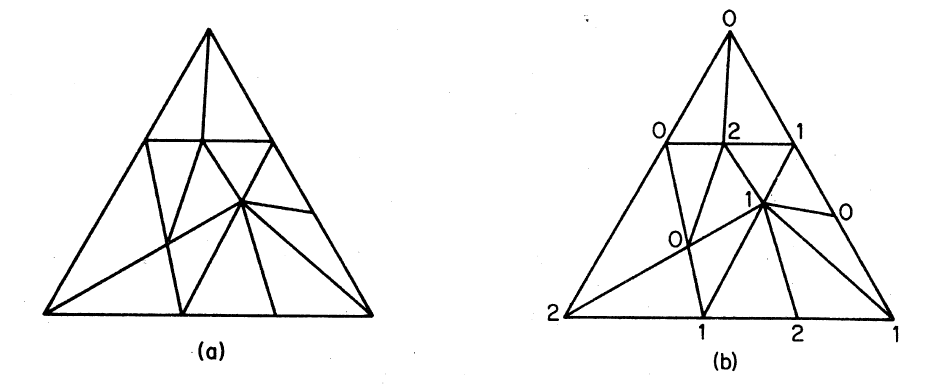
\includegraphics[scale=0.5]{simp.png}
    \caption{(a) Asimplicial subdivision of a triangle (b) a proper labelling of the    subdivision}
\end{figure}



\begin{itemize}
    \item T의 세개의 정점에는 0,1,2가 하나씩 붙는다.
    \item 그리고 T의 정점 사이의 정점에는 양 끝 T의 정점의 두 값만 값이 붙을 수 있다.
\end{itemize}
각 정점을 0,1,2로 가지는 삼각형을 구별된 삼각형이라한다.

\begin{theorem}[Sperner's lemma]
    적절히 분류되고(properly labelled) 단순하게(simplicial) 삼각형을 쪼갠것은 내부에 홀수개의 구별된 삼각형을 가진다.
\end{theorem}

\begin{proof}
    $T$를 $T_0$라 하자. 그다음 $T_1,T_2,...,T_n$을 쪼개진 삼각형들이라고 하자. 
    0과 1로 각각 분류된 $T_i$와 $T_j$가 공통 간선일때 $v_i$,$v_j$에 간선이 존재하는
    정점 집합 $\{v_0,v_1, ... ,v_n \}$을 정의하자.(이 정점은 T에 대응할수있다.)
    
    이 그래프에서 $v_0$는 명백하게 차수가 홀수값을 가진다.(1.9.1) 
    따라서 $v_1,v_2,...,v_n$중에 홀수개가 홀수값 차수를 가지게 된다.
    삼각형이라서 이 홀수개의 차수를 가지는 정점들이 차수값이 오직 1만을 가짐을 알 수 있다.
    $v_i$의 차수가 1임은 $T_i $가 구별된 삼각형인 경우만이다.
\end{proof}

\subsubsection{}
%191




week 4
\section{Tree}
\subsection{Trees}

\begin{dfn}[tree] connected acyclic graph

    acyclic graph : 사이클이 없는 그래프
\end{dfn}

\subsubsection{} 
%
\subsubsection{} 
%
\subsubsection{} 
%
\subsubsection{} 
%
\subsubsection{} 
%  2.1.5
Let 0 be a graph with v-I edges. Show that the following three statements are equivalent: 
(a) G is connected;
(b) G is acyclic;
(c) G is a tree.

연결된 acyclic graph는 정의에 의해 tree임이 자명하므로 간선의 개수가 $\nu -1$  일때, acyclic graph일때 connected한것과 connected graph일때 acyclic 그래프임이 필요충분조건임을 보이는 것으로 충분하다.

acyclic $\rightarrow$ connected graph

acyclic그래프가 connected graph가 아니라고 가정해보자.

그러면 각 component는 connected graph이므로 트리이다.
각 component의 간선의 갯수의 합은 $v(G_1)-1 + v(G_2)-1 + ... + v(G_n)-1 \neq v(G)-1 $
따라서 가정에 모순 다음 명제가 성립한다.

connected graph $\rightarrow$ acyclic

acyclic graph가 아니라고 하자 cycle이 형성된곳의 간선을 하나씩 제거해서 acyclic 그래프가 되도록 만들면 트리가 된다.
$\nu-1-n \neq \nu -1 $ 가정에 모순이라 다음 명제가 성립한다.
\subsubsection{} 
%
\subsubsection{} 
%
\subsubsection{} 
% 2.1.8
A centre of G is a vertex u such that max d(u, v) is as small as possible.
Show that a tree has either exactly one centre or two,
adj acent, centres.


G의 중심은 최대 d(u, v)가 가능한 한 작은 꼭지점 u이다.

트리 하나가 정확히 하나의 중심 또는 두 개의 인접한 중심을 가지고 있음을 보여라

week5

\begin{dfn}[spanning tree]
    그래프 $G$의 트리인 spanning subgraph를 $G$의 신장 트리(spaning tree)라고 부른다.
\end{dfn}

\begin{corollary}
    $2.4.1$ 모든 연결된 그래프는 스패닝 트리를 가진다.
\end{corollary}

\begin{proof}
    그래프 $G$가 connected graph이면 $G$의 cennected spanning subgraph가 존재한다.
    그래프 $H$를 $G$의 최소한의 connected spanning subgraph라 하자.
    이때 $H$가 acyclic가 아니라고 가정 해보자.
    그래프 $H$가 사이클이 존재하는 경우,간선 사이클 경로의 임의의 인접한 정점 $u, v$를 잡았을때 $u, v$의 간선을 제거해도 $u, v$는 여전이 연결되어있다. 이는 최소한의 connected spanning subgraph라는 것에 모순이다. 
    따라서 그래프 $H$는 connected spaning graph이며 acyclic함으로 스패닝 트리이다.
\end{proof}

\begin{theorem}
    $T$가 연결된 그래프 $G$의 스패닝 트리라고 하고 $e$를 $T$에 속하지 않은 $G$의 에지라고 하자. 그러면 $T + e$는 유일한 사이클을 가진다.
\end{theorem}
\begin{proof}
    $\psi_G(e) = xy$라 할때, 유일한 사이클이아닌 두 개 이상의 사이클이 생성될 경우  e의 에지 추가하기전의 $x, y$ 유일한 경로가아닌 두개이상의 경로가 있다는 것을 의미하는데 트리는 유일한 경로임이 이미 증명되었으므로 유일한 사이클을 가진다.
\end{proof}
\subsection{Cut Edges and Bonds}

\subsection{Cut Vertices}

\subsection{Cayley's Formula}
\begin{dfn}[contract]
    그래프 $G$의 한 에지$e$를 수축한다는 것은 에지 $e$를 그래프에서 삭제하고 양 끝점을 하나의 정점으로 합치는 것이다. 그 결과 만들어지는 그래프를 $G \cdot e$로 표시한다.
    \begin{itemize}
        \item $\nu(G \cdot e) = \nu(G \cdot e) - 1$
        \item $\varepsilon(G \cdot e) = \varepsilon(G \cdot e)-1$
        \item $\omega(G \cdot e) = \omega(G)$
        \item  $T$가 트리이면 $T \cdot e$도 트리이다.
        \item 그래프 G의 스패닝 트리의 개수를 $\tau(G)$로 표시한다.
    \end{itemize}
\end{dfn}

\begin{theorem}
    2.8 그래프 $G$의 임의의 에지 $e$에 대해서 $\tau(G) =\tau(G-e) + \tau(G \cdot e)$이 성립한다.
\end{theorem}

\begin{proof}
    그래프 $G$에서 에지$e$를 포함하지 않는 스패닝 트리는 $G-e$의 스패닝 트리 또한 된다.
    따라서 $\tau(G-e)$는 그래프 $G$에서 에지 $e$를 포함하지 않는 스패닝 트리의 개수와 같다.
    에지 $e$를 포함하는 $G$의 임의의 스패닝 트리 $T$는 $G \cdot e$의 스패닝 트리 $T \cdot e$에 일대일 대응한다.(추가적인 논리 필요) 따라서 $\tau(G \cdot e)$는 $G$에서 에지 $e$를 포함하는 스패닝 트리의 개수이다. 따라서 정리가 성립한다.
\end{proof}


Fortunately, and rather surprisingly, there is a closed formula for T(G) which expresses T(G) as a determinant; 
we shall present this result in chapter 12.


\begin{theorem}
    $Cayley's folmula$ : $\tau(K_n)= n^{n-2}$
\end{theorem}

\begin{proof}
    $K_n$의 정점 집합을 $N = \{1,2, ...,n\}$라 놓자.
    그러면 $n^{n-2}$는  $N$으로부터 길이가 $n-2$인 수열\footnote{$Pr\ddot{u}fer \: sequences$라 한다.}을 만드는 수로 볼 수 있다.
    따라서 이 수열이 $K_n$의 spanning tree와 1:1대응을 하는걸로 이 증명이 완성된다.
    $K_n$의 spanning tree $T$에 대해서 특정 수열 ${t_1, t_2, ... , t_{n-2}}$과 연관지으려 한다.
    $N$을 정렬된 셋이라 가정하고, $s_1$은 $T$의 차수가 1인 첫번째 정점이라하자. $s_1$은 $t_1$과 인접한 정점이다.
    그다음에 $s_1$를 $T$에서 제거하자 그다음 $T-s_1$에 차수가 1인 정점 한개를 $s_2$라 하자 이 짓거리를 $t_{n-2}$가 지워져 두 정점이 남을때 까지 반복한다. 총 반복은 $n-2$번 반복한다. 따라서 spanning tree가 수열에 대응함을 보였다.
    수열이 spanning tree에 대응함을 보이자.
    sequence P에 없는 1에서 n중 가장 작은 숫자를 찾아 P의 첫번째 숫자에 연결한다.
    그 후 P의 첫번째 숫자를 제거한다.
    P가 존재하지않을 때 까지 반복한다. 마지막 연결되는 숫자는 n이다.
    이렇게 함으로써 수열이 트리에 대응됨을 보일수있다.
    수열의 갯수가 $n^{n-2}$개 이므로 트리의 개수도 $n^{n-2}$개이다.
\end{proof}



    %https://academic.naver.com/article.naver?doc_id=13986337

    %https://en.wikipedia.org/wiki/Pr%C3%BCfer_sequence

    %http://blog.daum.net/eternaljk/6176142

    %    https://www.math.uchicago.edu/~may/VIGRE/VIGRE2006/PAPERS/Casarotto.pdf

\end{document}